\section{Main findings}
\paragraph{Fact 1: there are substantial differences in the \alert{level} of the gender gap across CZ}


Figure \ref{fig:gap_map2020} illustrates variation of the gender gap across US CZ in 2020. The figure restricts to CZ with population densities above 1 person per square kilometer in 1950. In 2020, men had an unconditional average wage 19
 (se 5
)
 log-points larger than women's. The map however, shows that there are wide variations from this average across CZ. Men's wage advantage is below 14 log-points in the Northeast and most of the West Coast, while it is above 24 log-points in the parts of the South West. The standard deviation in gender-wage gap across the 625 CZ shaded in the graph is of 5
log-points, which represents 26\%
of the average national gap.
 
 [make an argument here that these differences are economically significant]
 
 
 


\begin{figure}[!h]
\centering
\caption{The gender gap in the US in 2020}
\label{fig:gap_map2020}
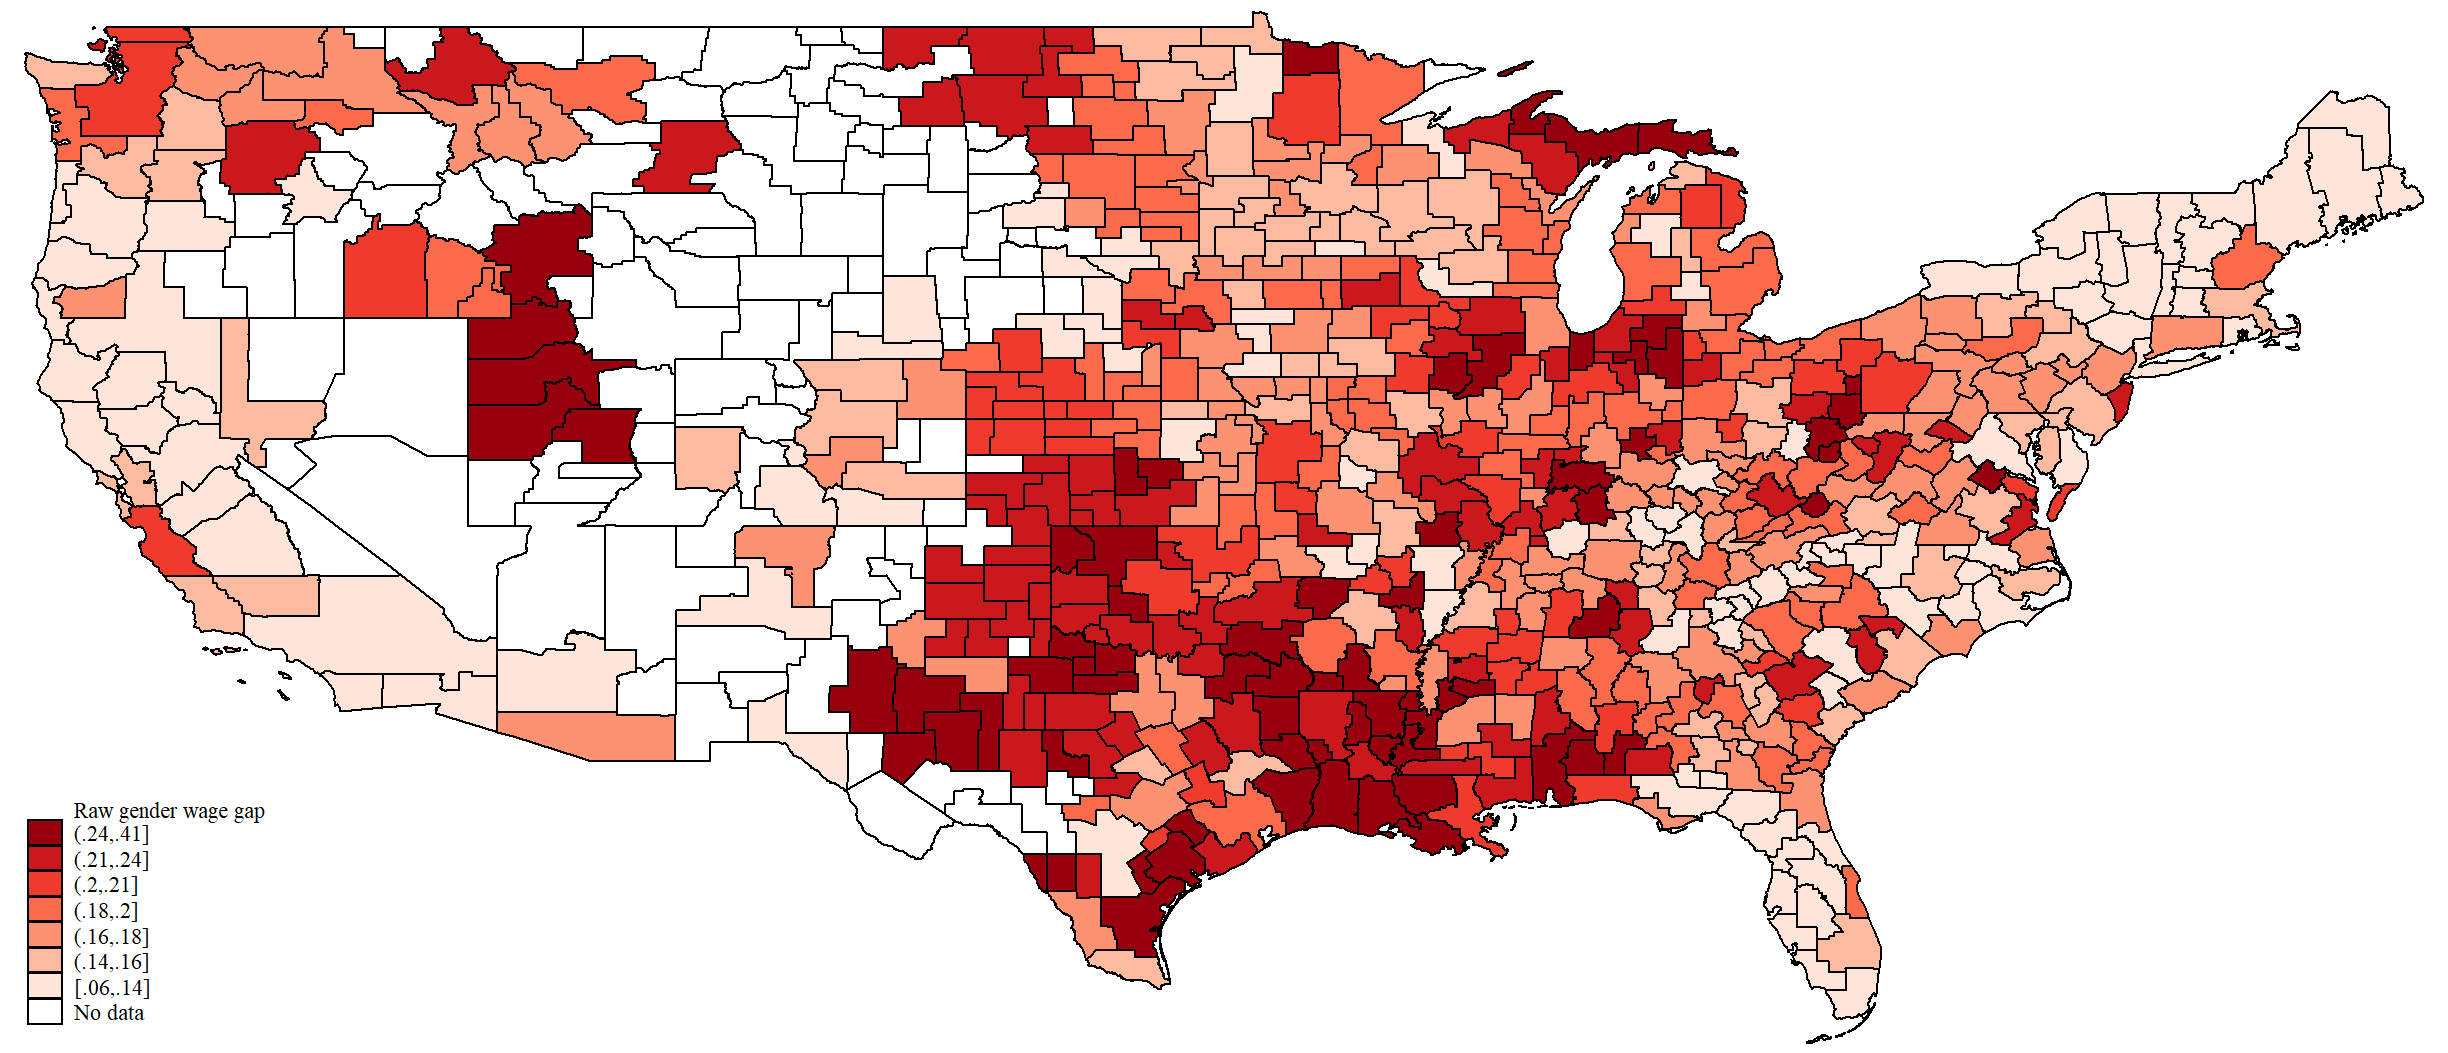
\includegraphics[width=1\textwidth]{../2_analysis/output/figures/raw_wage_map2020_full_time}
\par \begin{minipage}[h]{\textwidth}{\tiny\textbf{Note:} darker colors denote higher relative wages for men. Figure restricts to czones with population densities above 1 person per km$^2$ and full-time year-round workers.}\end{minipage}
\end{figure}



\paragraph{Fact 2: there are substantial differences in the \alert{evolution} of the gender gap across CZ}

\bitem	
	\item Take two CZ as an example and show the evolution of the gender gap in these two places.
	\item Then show statistics on the change of the gender gap across places.
\eitem 
\paragraph{Fact 3: the gender gap has decreased the most in the densest CZ}
	\begin{figure}[!h]
\centering
\caption{Change in male wage advantage in US CZ}
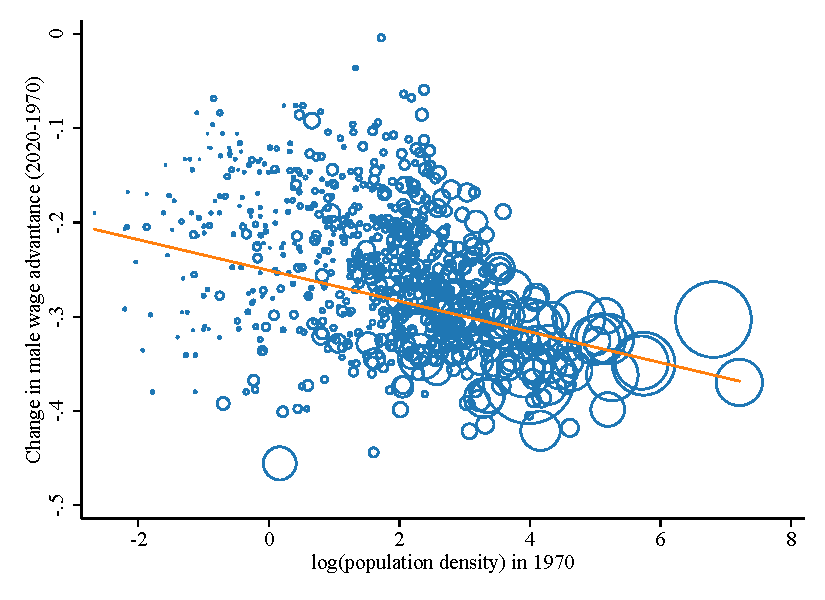
\includegraphics[width=.75\textwidth]{../2_analysis/output/figures/change_in_gap}
\end{figure}

	
	
	[add residualization at the individual level]

\paragraph{Fact 4: the relationship between population density and the gender gap has inverted over the period}

[write regression I am writing here]

[graph of cross-sectional slope goes here]
